\documentclass[12pt]{article}
\usepackage{lipsum}
\usepackage[utf8]{inputenc} 
\usepackage[T1]{fontenc}
\usepackage{lmodern}
\usepackage{graphicx}
\usepackage[french]{babel}


\newcounter{eqn}
\renewcommand*{\theeqn}{\alph{eqn})}
\newcommand{\num}{\refstepcounter{eqn}\text{\theeqn}\;}

\makeatletter
\newcommand{\putindeepbox}[2][0.7\baselineskip]{{%
    \setbox0=\hbox{#2}%
    \setbox0=\vbox{\noindent\hsize=\wd0\unhbox0}
    \@tempdima=\dp0
    \advance\@tempdima by \ht0
    \advance\@tempdima by -#1\relax
    \dp0=\@tempdima
    \ht0=#1\relax
    \box0
}}
\makeatother



\begin{document}

\title{Chapitre 1 : G\'eneralit\'e}
\date{}
\maketitle

\setcounter{section}{+1}
\subsection{introduction}
\paragraph{} 
Il est bien simple et évident pour nous, humains, de reconnaitre ce que nous voyons quasi instantanément.  Cependant, pour un ordinateur, c’est une toute autre histoire. Etant donnée la puissance et la complexité de notre cerveau,  les traitements s’y faisant nous sont très difficile à comprendre, et autant plus difficile à recréer. 
\paragraph{}
Si on prend en exemple l’objet de notre étude qui est la reconnaissance des textures et qui elle, est une partie du traitement d’images, nous nous retrouvons dans le paradoxe de l’étude d’une entité non défini mais parfaitement reconnaissable. Le fait de reconnaitre un ciel bleu et le distinguer d’une rivière ou des roches tout au tour est élémentaire  pour le cerveau humain et très utilisé par ce dernier. On peut aussi très facilement distinguer une table en plastique d’une table en bois. Cependant, la simple définition du  terme « texture » nous reste inconnu. 

\subsection{Définition de la texture}
\paragraph{}
Plusieurs tentatives de la définir ont été regroupées dans un catalogue par Coggins [1]. On peut en prendre quelques exemples:

\subparagraph{
"Nous pouvons considérer une texture comme ce qui constitue une région macroscopique. Sa structure est simplement attribuable aux motifs répétitifs dans lesquels des éléments ou des primitives sont disposées selon une règle de placement "
}

\subparagraph{
 "La texture est défini pour nos fins comme un attribut d'un domaine n'ayant aucune composante qui apparaissent dénombrable. Les relations de phase entre les composants ne sont donc pas apparentes. Le terrain ne devrait pas contenir un gradient évident. Le but de cette définition est d'attirer l'attention de l'observateur sur les propriétés globales de l'affichage -. C'est à dire sa "rudesse" globale "bosselage", ou "finesse". Physiquement, les modèles innombrables (apériodiques) sont générés par stochastique par opposition de processus déterministes. A la perception, cependant, l'ensemble des motifs sans composants énumérables évidentes comprendra de nombreux (et même périodique) textures déterministe."
}

\subparagraph{
"La texture est une notion apparemment paradoxale. D'une part, elle est couramment utilisée dans le traitement de l'information visuelle, surtout pour des raisons pratiques de classification. D'autre part, personne n'a réussi à produire une définition communément acceptée de la texture. La résolution de ce paradoxe, dépendra d'un modèle plus riche, plus développé pour le début de traitement de l'information visuelle, un aspect central de ce qui sera un systèmes représentatif à différents niveaux d'abstraction. Ces niveaux vont probablement inclure intensités actuels au fond et progresseront à travers des pointes et des descripteurs d’orientation vers la surface, et peut-être des descripteurs volumétriques. Compte tenu de ces structures multi-niveaux, il semble clair qu'ils doivent être inclus dans la définition, et dans le calcul, des  descripteurs de la texture."
}

\subparagraph{
" La notion de texture semble dépendre de trois ingrédients: (1) un certains « ordre » local répété sur une région qui est grande par rapport à la taille de l'ordre, (2) l'ordre consiste en l'arrangement non aléatoire de pièces élémentaires et (3) les parties sont des entités plus ou moins uniformes ayant approximativement les mêmes dimensions partout dans la région texturée. "\\\\
}


Figure 1: Tigre dans une forêt				         Figure 2: Bétons

\paragraph{}
Quelques paramètres essentiels sont à prendre en compte dans l’étude des textures. Si on prend par exemple la photo d’une forêt, on pourra distinguer la terre comme texture,  l’ensemble des feuille d’un arbre comme une autre, mais encore la peau d’un tigre [Figure 1].
Si on prend par contre une prise aérienne de cette même foret, on pourra considérer le tout comme une seule texture qui se différenciera de la texture formé par les bâtiments d’un village par exemple. 
Aussi, le voisinage d’une texture joue un grand rôle dans l’interprétation de cette dernière. Une couche de béton par exemple seul peut avoir plusieurs interprétations, elle peut être une partie d’un mur,  un banc, le sol ou  bien des marches d’escalier [Figure 2].
Notons aussi que certaine structure ont une dynamique importante au fil du temps qui fait varier leur apparence. Par exemple un ciel bleu avec quelque nuage (le vent fera constamment varier la forme des nuages). 

\subsection{Segmentation d’images :}

Dans le traitement d’image, une des plus grandes préoccupations est la segmentation d’images. C’est, comme son nom l’indique, le processus de partitionnement d’image digitale en différentes partie et ce, pour simplifier ou la « compréhension »  de cette dernière par la machine, et la rendre plus facilement analysable.

Le principe est de reconnaitre des objets ou des frontières. Le but étant de donner une signification aux pixels de l’image. Elle est utilisé généralement dans :

\begin{figure}
\begin{tabular}{cccc}

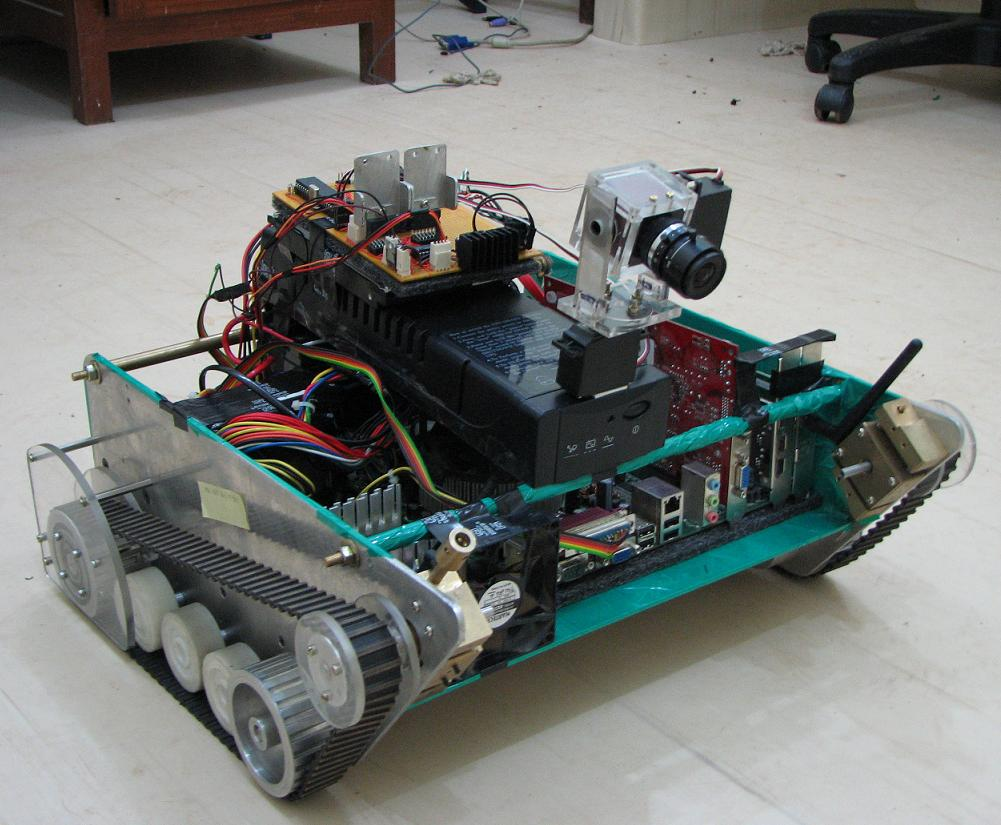
\includegraphics[width=6cm, height=4.5cm]{pics/VisionArtificielle1.jpg}
&
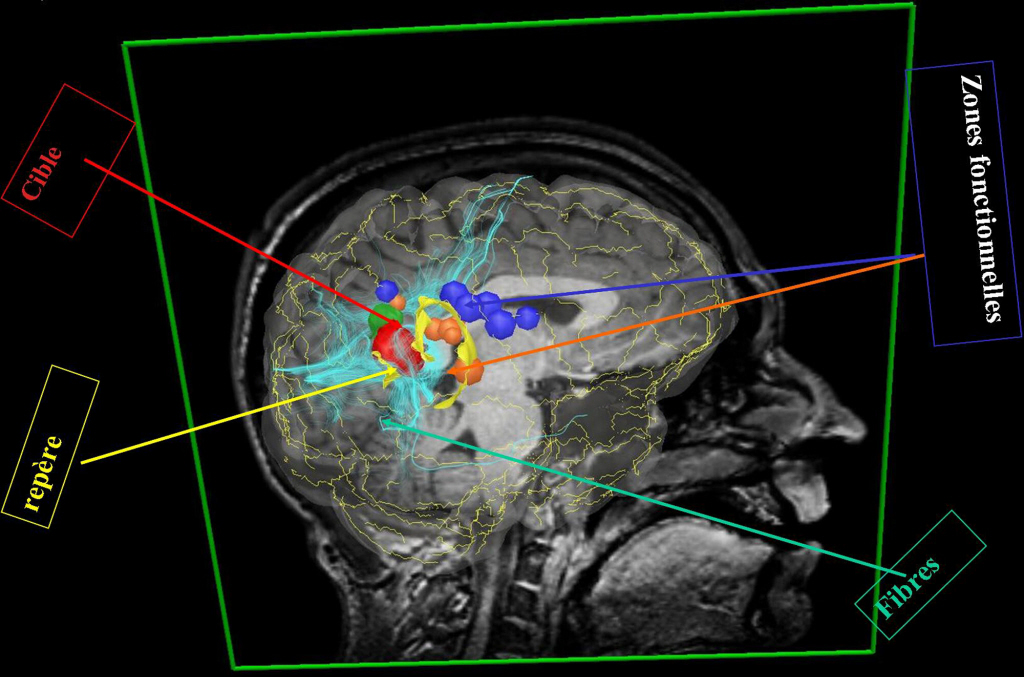
\includegraphics[width=6cm, height=4.5cm]{pics/ImagerieMedical.jpeg}\\
Figure 3.a & Figure 3.b\\\\

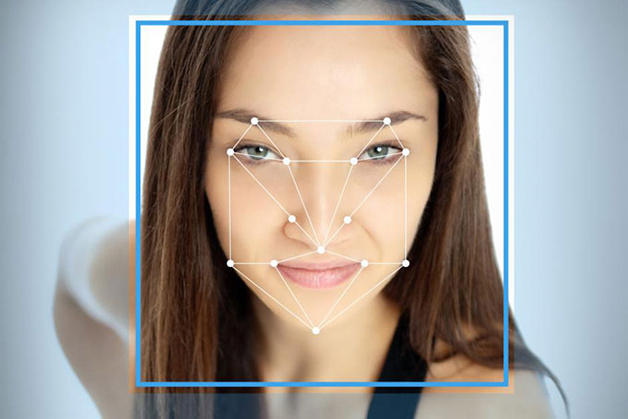
\includegraphics[width=6cm, height=4.5cm]{pics/reconaissanceFacial.jpg}
&

\includegraphics[width=6cm, height=4.5cm]{pics/empreinteDigitale.jpeg}\\
Figure 3.c & Figure 3.d\\\\

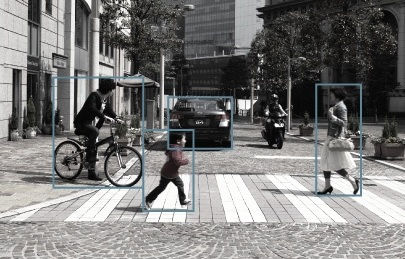
\includegraphics[width=6cm, height=4.5cm]{pics/DetectionPieton.png}
&
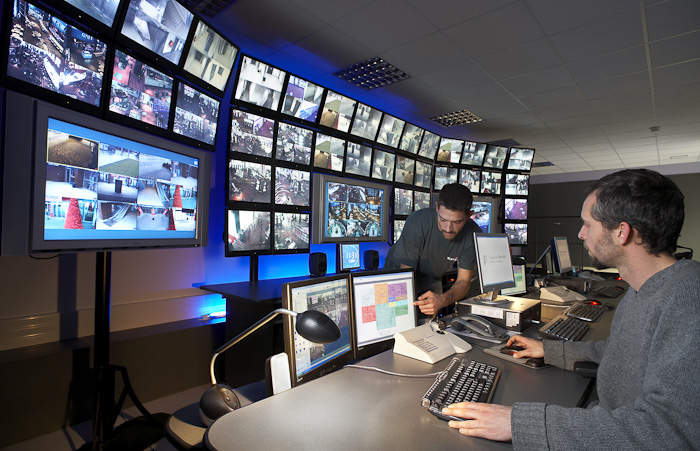
\includegraphics[width=6cm, height=4.5cm]{pics/videoSurveil.jpeg}\\
Figure 3.e & Figure 3.f\\\\

\multicolumn{2}{c}{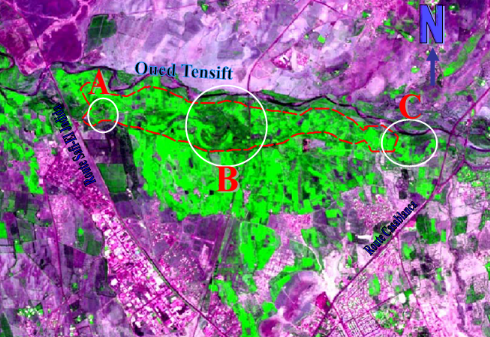
\includegraphics[width=6cm, height=4.5cm]{pics/Satellite.png}}\\
\multicolumn{2}{c}{Figure 3.g}\\


\end{tabular}
\end{figure}

\indent La vision artificielle (Figure 3.a)\\
L’imagerie médicale (Figure 3.b)\\
La reconnaissance faciale (Figure 3.c)\\
La reconnaissance d'empreintes digitales (Figure 3.d)\\
La détection de piétons (Figure 3.e)\\
La vidéo surveillance (Figure 3.f)\\
Localiser des objets dans des images satellitaires (Figure 3.g)\\

\subsection{Les approches analytiques :}

On retrouve principalement quatre (4) approches analytiques de texture qui sont :
Approche structurelle (ou fréquentielle): Ces méthodes supposent que les textures sont formées d’éléments structurants de base. L’idée générale de ces méthodes est une recherche et une description des éléments structurants suivie d’une étude de la répartition spatiale de ces derniers [3].

Approche statistique : Ici, la texture est définie selon la distribution des niveaux de gris dans l’image, et c’est sur quoi cette méthode se base.

Approche modèle : Elle se repose sur l’utilisation de fractals et de modèles stochastique.

Approche transformée (méthodes de traitement du signale): Des recherches de  psychophysique ont démontrés que le cerveau humain fait une analyse de fréquence des images. 

L’utilisation de ces approches diffère selon le type de texture. Ces dernières se regroupent en trois différentes catégories : structurelle, aléatoire ou directionnelles.











\subsubsection{Textures structurelles}
				

Figure 4 : Textures structurelles (péridique)

\paragraph{}
La figure 4 présente un premier type de textures dites structurelles.
On les appelle ainsi car on peut les considérer comme étant la répartition spatiale de motifs élémentaires de base dans différentes directions de l’espace suivant une certaine règle de placement. En effet, on s’aperçoit que la première représente un mur de brique, elle est composée d’un ensemble d’éléments de base (les briques) disposés relativement régulièrement de manière horizontale. La deuxième texture est aussi composée de motifs de base alvéolés agencés d’une manière particulière les uns à côté des autres[3].
Cette catégorie de textures a engendré des méthodes d’analyse dites structurelles.

\subsubsection{Textures aléatoires}

	 		

Figure 5 : Textures aléatoires

\paragraph{}
Le deuxième type de textures est exposé dans la figure 5. Contrairement aux deux premières, celles-ci ont un aspect anarchique tout en restant globalement homogènes. On ne peut pas en extraire de motifs de base se répétant spatialement. On les appelle des textures aléatoires.
Cette catégorie a fourni d’autres travaux de recherches plutôt fondés sur des méthodes
d’analyse statistique[3].

\subsubsection{Textures directionnelles}

              

Figure 6 : Textures directionnelles

\paragraph{}
Les textures directionnelles (Figure 6) ne sont pas forcément aléatoires et ne présentent pas d’éléments structurants de base.
On peut les décrire de manière générale comme étant des textures  présentant des structures orientée selon une direction privilégiée..
Les textures directionnelles se caractérisent soit par leur orientation globale, soit par un champ d’orientations locales. par exemple La texture de gauche de la figure 6 laisse apparaître des lignes obliques, et celle au milieu possède des lignes verticales.
Dans les textures directionnelles réelles, le champ d’orientation n’est en effet pas toujours uniforme comme la texture de droite de la figure 6.

\paragraph{}
Ces différentes catégories de textures nous montrent qu’il est difficile d’en donner une
définition précise. Les définitions semblent s’adapter aux différents types de textures : l’une
donne une information structurelle, déterministe et constructive (identification de la texture

Nous nous allons nous approfondir sur l’approche statistique étant donné qu’elle sera celle qu’on implémentera dans nôtre étude.
Plus précisément, nous parlerons des deux méthodes suivantes : 

\subsubsection*{A)- Matrice de cooccurrence :} (ce qui est entre [] est un vecteur)
L’analyse des textures se base très généralement sur l’utilisation de la matrice de cooccurrence.
Une image « I » est une matrice de « n » lignes et « m » colonnes. « f(i,j) » défini le niveau de gris du pixel présent en ligne « i » et  colonne « j ». « Ng » est le nombres de niveaux de gris de « I ».
La matrice M-I-[d] de cooccurrence (ou Gray Level Co-occurrence Matrix - GLCM) est une matrice carrée de taille « Ng x Ng », et est définie en fonction de l’image « I » et du vecteur de déplacement :\\

[d]= [$\Delta i, \Delta j$] défini, lui par l’angle $\emptyset$ (=0\char23 | 45\char23 | 90\char23 | 135\char23)  et par la distance « d » entre deux pixels.
\\
Pour tout « (i,j) dans $R^2$ » :

$$M_{I[d]} (i,j) = card\{ (k1,l1),(k2,l2) \}$$
$$Où: f(k1,l1)=i , f(k2,l2)=j, [(k2,l2)] - [(k1,l1)]=[d]$$\\


En d’autres termes, on s’intéresse au nombre d’apparition des couples de niveau de gris « i,j » construisant un vecteur [d].

\begin{figure}
\centering
\includegraphics[width=8cm]{pics/GLCM.jpg}
\caption{ Figure 7 : Exemple de construction d’une matrice de cooccurrence}
\end{figure}


Etant donné que la taille de la matrice dépend du nombre de niveaux de gris, celle-ci peut atteindre un taille de 256 x 256, ce qui est bien évidement trop immense pour penser à exploiter cette dernière directement. C’est pour cela que Harlick et al [] ont proposé 14 paramètres pour mieux exploiter les informations fournies par cette matrice.
Les six qui sont les plus utilisé sont : []
L’énergie: permet de mesurer l’uniformité de la texture.\\

ENE$=\sum\limits_{i}\sum\limits_{j} (P_{ij}(\delta,\theta)^2)$\\

Le contraste: permet de  mesurer la variation locale de niveau de gris.\\

CST$=\sum\limits_{i}\sum\limits_{j} ((i-j)^2 P_{ij}(\delta,\theta))$\\

La variance: permet d’évaluer l’intensité de variation de niveau de gris par rapport au niveau moyen.\\

VAR$=\sum\limits_{i}\sum\limits_{j} ((i-\mu)^2 P_{ij}(\delta,\theta))$\\

L’entropie : permet de mesurer le désordre dans une image, ou a quel point la texture est aléatoire.\\

ENT$= - \sum\limits_{i}\sum\limits_{j} (log P_{ij}(\delta,\theta) P_{ij}(\delta,\theta))$\\

La corrélation: mesure  les dépendances linéaires entre les lignes et les colonnes dans l’image.\\

COR = $\sum\limits_{i}\sum\limits_{j} (\frac{P_{ij}(\delta,\theta)(i-\mu)(j-\mu)}{\delta^2}) $\\

Le moment inverse : mesure l’homogénéité de l’image.\\

IDM = $\sum\limits_{i}\sum\limits_{j} (\frac{P_{ij}(\delta,\theta)}{1+(j-i)^2})$\\

\subsubsection*{B)- Motif binaire local (LBP-Local Binary Pattern):}
Cette méthode présente un énorme avantage par sa simplicité de calcul. Elle permet de décrire la texture avec deux propriétés: Le contraste, et la configuration spatiale locale. 
Le principe de calcule de ces deux propriétés se base sur la comparaison d’un pixel au centre avec ces 8 voisins en prenant des matrices de 3x3 pixels .
On calcule le contraste en appliquant la formule suivante : 

Où les « Hi » représentent les valeurs de niveau de gris des voisins supérieur à celui du centre, et Nh le nombre de ces valeurs. Et les « Li » représentent les valeurs de niveau de gris des voisins inférieure à celui du centre, et Nl le nombre de ces valeurs.
Pour la méthode motif binaire local, on compare le pixel du centre avec ses voisins, on génère une matrice de « seuillage »  où : si la niveau de gris du voisin est supérieur a celui du centre la valeur de ce premier sera égale à 1. Elle est égale à 0 sinon.
On créera aussi une matrice de « seuillage »  qui sera remplis d’en haut à gauche en suivant le sens des  aiguilles d’une montre par les puissances de deux.
On aura un résultat comme suit :

Figure 8 : Calcul du motif binaire

En lisant les valeurs de la matrice obtenu d’en haut à gauche en suivant le sens des  aiguilles d’une montre on obtient un code binaire appelé « motif ». Ce code binaire est ensuite converti en décimale en multipliant la matrice « seuillage » par la matrice de « poids », ce qui nous donne la valeur de LBP suivante :
$
motif = 10000111 \\
LBP = 1 +32 + 64 + 128 = 225 \\
$
On aura ainsi la nouvelle valeur du niveau de gris du pixels et ses voisins, on remplace le niveau de gris du pixels centrale de la matrice par le niveau de gris égale au résultat trouvé précédemment.\\



Figure 9 : Transformation LBP de l'image\\


On définie aussi une valeur "U" qu'on appellera valeur de « transition » qui sera égale au nombre de transitions de 0 vers 1 et de 1 vers 0 qu'on trouve dans la valeur du « motif » comme suit :\\



Figure 10 : Extraction du nombre U à partir du motif\\


En réalité, tous les « motifs » (256) ne sont pas importants
Ceux qui ont un nombre de transition U=2 and U=0, sont appelé « uniform patterns ». Mäenpää et al. A trouvé qu’un nombre moins important de ces derniers sont plus résistant aux transformations géométriques telle que la rotation [10]. Ils ont proposé l’utilisation de 58 « uniform patterns » composés de (00000000, 11111111), (00000001, 00000011, 00000111, 00001111, 00011111, 00111111, 01111111) [11]
Pour étudier l’uniformité, on construit un histogramme qui rassemble les 256 possibilités (ou des 58 défini ci-dessus) et calcule leurs occurrences pour enfin faire une étude statistique sur ce premier.\\



\section*{Ref :}
1- Coggins, J. M., “A Framework for Texture Analysis Based on Spatial Filtering,” Ph.D. Thesis, Computer Science Department, Michigan State University, East Lansing, Michigan, 1982.
H.Majdoulayne 2009:  Extraction de caractéristiques de texture pour la classification d'images satellites", thèse de doctorat, université de Toulouse, France. 
[10] Zhenhua Guo; Lei Zhang; Zhang, D.; , "A Completed Modeling of Local Binary Pattern Operator for Texture Classification," Image Processing, IEEE Transactions on , vol.19, no.6, pp.1657-1663, June 2010.
[11] Doc de Izem

\end{document}
